\documentclass{article}
\usepackage{amsmath, fullpage}
\usepackage{graphicx}
\usepackage[portuguese]{babel}
\graphicspath{{imgs/}}
\begin{document}

\title{Experimentos finais de química}
\author{Henrique Bernardes}
%\date{\vspace{-5ex}}
\maketitle
\thispagestyle{empty}
\section{Primeiro Experimento - Calorimetria}

A termodinâmica é o estudo das transformações de energia e se baseia em duas leis ahisdhioashdoi:
\begin{itemize}
  \item A energia não é destruida, ela é conservada. Durante um processo, ela é transformada de um tipo para outro.
  \item Entropria - mede o grau de desorganização das partículas em um sistema. Um processo somente ocorre se a entropia total do sistema aumenta, ou seja, o grau de desordem aumenta.
\end{itemize}
Temos também que, a variação de energia interna de um sistema($\Delta U$) é o resultado de dois tipos de transferência de energia: calor e trabalho.
\begin{align}
  \Delta U = Q - W
  \label{eq:primeiraLei}
\end{align}
Se o volume é constante, temos que $\Delta U = Q$, ou seja, em um sistema com volume constante, podemos medir a entalpia apenas observando a troca de energia(na forma de calor) entre ele e a vizinhança.

\subsection{Entalpia}
Temos, também, a entalpia(H), utilizada nos estudos e nas transformações das reações químicas.
Da primeira lei temos a fórmula \ref{eq:primeiraLei}; agora, precisamos explicitar a fórmula do trabalho:

\begin{equation}
  W=\int_{V_0}^{V} p\, dV  
\end{equation}
aplicando um diferencial de ambos os lados:
\begin{align*}
    \delta W=pdV
\end{align*}
aplicando à formula \ref{eq:primeiraLei} em forma diferencial, obtemos:
\begin{align}
    dU=dQ-pdV
  \label{eq:primeiraLei2}
\end{align}
sabemos, também de fenômenos de transporte que:
\begin{equation}
  H=U+pV
  \label{eq:leiEntalpia}
\end{equation}
Observando a relação dada pela fórmula \ref{eq:primeiraLei2} e aplicando à equação \ref{eq:leiEntalpia}, temos:
\begin{align*}
  dH&=dU + d(pV)\\
  &=\delta Q -pdV + (Vdp)+(pdV) \\
  &=\delta Q +(Vdp)\\
\end{align*}
assumimos então o caso de pressão constante, logo, $dp=0$:
\begin{align}
  dH=\delta Q 
\end{align}
Dessa forma, conhecendo a equação para o cálculo da variação da entalpia, pode-se calcular o calor trocado durante o processo. Por isso, reações podem ser classificadas da seguinte forma:
\begin{enumerate}
  \item $\Delta H_r < 0$ são reações exotérmica, ou seja, emitem calor;
  \item $\Delta H_r > 0$ são reações endotérmicas, ou seja, absorvem calor.
\end{enumerate}

\section{Terminologias}
\subsection{Capacidade Calorífica}
A \textbf{capacidade calorífica}(C) de um objeto é a razão entre o calor fornecido e o aumento de temperatura observado:
\begin{equation}
  C=\frac{q}{\Delta T}  
  \label{eq:eqCapCalorifica}
\end{equation}
e, por consequência, $q=C \Delta T$, onde C pode também ser chamado de capacidade térmica. Portante, a capacidade térmica mede a quantidade de calor necessária para que haja uma variação unitária de temperatura. 

\subsection{Calor específico}
Mede o calor necessário para que haja uma variação unitária de temperatura de uma massa unitária de uma certa substância, ou seja:
\begin{equation}
  c=\frac{q}{m\Delta T }
  \label{eq:eqCalorEspecifico}
\end{equation}
ou seja, $q=cm\Delta T$. A transferência de energia na forma de calor é medida com um calorímetro. Este é um sistema fechado no qual o calor transferido é monitorado pela variação de temperatura que ele provoca, utilizando a capacidade calorífica do calorímetro($C_{cal}$) para converter a mudança de temperatura em calor produzido.
A capacidade calorífica do calorímetro pode ser obtida experimentalmente através do métodos das mistúras: aquecendo uma quantiade de água a uma temperatura maior que a da água contida no calorímetro e as misturando, fazendo a água com temperatura maior ceder calor á agua com temperatura menor e ao calorímetro.
\begin{equation}
  C(T_{eq}-T_1)+m_1+c_1(T_{eq}-T_1)=m_2c_2(T_2-T_{eq})
\end{equation}

Isso é possível devido ao equilíbrio térmico que é atinjido, ou seja, uma quantidade de energia térmica é transferida da substãncia de maior temperatura para a de menor temperatura, associada à quantidade de calor que a substância de menor energia irá receber. Pelo princípio da conservação de energia:
\begin{align}
  q_{ganho}=q_{perdido}
\end{align}
\newpage
Neste experimento, o calorímetro é formado por um recipiente interno(béquer) revestido por um copo isopor com finalidade de eliminar a propagação de calor para o ambiente externo.
\begin{figure}[!h]
  \centering
  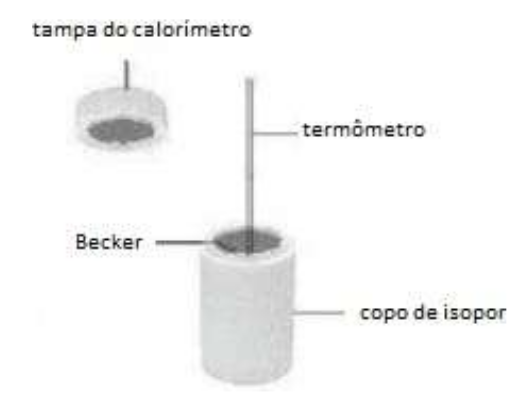
\includegraphics[width=0.2\linewidth]{calorimetro.png}
  \caption{Calorímetro}
  \label{fig:Calorimetro}
\end{figure}
Após a determinação da capacidade calorífica do calorímetro é possível converter em variação de energia o aumento ou diminuição da temperatura provocada pela reação química:
\begin{equation}
  q_{cal}=C_{cal}\Delta T
  \label{eq:eqCalorimetro1}
\end{equation}
Como o calor gerado na reação será transferido para o calorímetro, podemos considerar $q_{reacao}=q_{calorimetro}$. Se não houver trabalho de expansão(ou seja, a volume constante) $\Delta U = q_{reacao}$ e, portanto, podemos dizer que $\Delta U = q_{reacao} = -q_{cal}$. Assim sendo, é possível determinar a variação da energia interna da reação:

\begin{equation}
  \Delta U = - C_{cal} \Delta T
  \label{eq:eqCalorimetro2}
\end{equation}

\subsection{Observações}
Calor de neutralização é a quantidade de calor liberada quando um ácido e uma base reagem para formar sal e água, ou seja, uma reação de neutralização.
\section{Segundo experimento - Cinética Química} 
A reação de Landolt, conhecida como a "reação do relógio de iodo", trata-se da reação entre os \textbf{íons bissulfito e iodato em meio ácido, com formação de iodo}. Na realidade, o mecanismo dessa reação não é trivial, envolvendo, envolvendo várias etapas com velocidades distintas, durante as quais espécies intermediárias são formadas e posteriormente consumidas. Todavia, é possível representar a equação de Landolt por meio de três equações básicas apresentadas à seguir.


Inicialmente, o bissulfito ($HSO_{3}$), reage com iodato($IO_{3}$), formando bissulfato($HSO_{4}$) e iodeto(I):
\begin{center}
  Etapa Lenta
\end{center}
\begin{equation}
  3HSO_{3(aq)} + IO_{3(aq)} \rightarrow 3HSO_{4(aq)}+I_{(aq)} 
  \label{eq:eq1}
\end{equation}
a medida que o iodeto vai sendo formado lentamente, este reage rapidamente com o iodato, ainda presente em grande quantidade, gerando iodo elementar($I_2$):
\begin{center} 
  Etapa Rápida
\end{center}
\begin{equation}
  5I_{(aq)} + IO_{3(aq)} + 6H_{(aq)} \rightarrow 3I_2 + 3H_2O
  \label{eq:eq2}
\end{equation}
enquanto houver bissulfito na solução, este consumirá imediatamente o iodo formado, produzindo novamente iodeto:
\newpage
\begin{center}
Reação muito rápida
\end{center}
\begin{equation}
  3HSO_{3(aq)}+I_2+H_2O \rightarrow HSO_{4(aq)}+3H_{(aq)}
  \label{eq:eq3}
\end{equation}
Assim sendo, o iodo somente será observado quando todo o bissulfito tiver sido consumido.
O tempo transcorrido a partir do momento da mistura dos reagentes(bissulfito e iodato) até o aparecimento do iodo é um parâmetro de fácil medição, o qual permite avaliar como a velocidade da reação de Landolt pode variar em diferentes condições experimentais. Uma concentração mínima de iodo poderá ser sensivelmente detectada se houver amido presente no meio reacional, pois este forma um complexo de intensa coloração azul com o iodo.
O objetivo deste experimento será observar o tempo necessário para a formação do iodo na reação de Landolt, variando-se a concentração dos reagentes e a temperatura(mostrar o efeito da concentração dos reagentes e da temperatura sobre a velocidade das reações).
\subsection{Observações}
A função do amido na reação de Landolt é como indicador: indicando quando o iodo começa a ser formado, formando um complexo de intensa coloração azul com o iodo.
Os diferentes fatores que afetam a velocidade das reações são 
\begin{enumerate}
  \item Concentração dos reagentes;
  \item Temperatura na qual a reação está submetida;
  \item Pressão;
  \item Presença de catalisadores. 
\end{enumerate}
A função de um catalisador é fornecer um caminho de menor energia de ativação(energia necessária para que uma reação ocorra)para uma reação, fazendo com que ela ocorra em um menor tempo/maior velocidade, sem ser consumido.


\end{document}
